Octagon $ABCDEFGH$ with side lengths $AB = CD = EF = GH = 10$ and $BC=  DE = FG = HA = 11$ is formed by removing four $6-8-10$ triangles from the corners of a $23\times 27$ rectangle with side $\overline{AH}$ on a short side of the rectangle, as shown. Let $J$ be the midpoint of $\overline{HA}$, and partition the octagon into $7$ triangles by drawing segments $\overline{JB}$, $\overline{JC}$, $\overline{JD}$, $\overline{JE}$, $\overline{JF}$, and $\overline{JG}$. Find the area of the convex polygon whose vertices are the centroids of these $7$ triangles.

\begin{center}
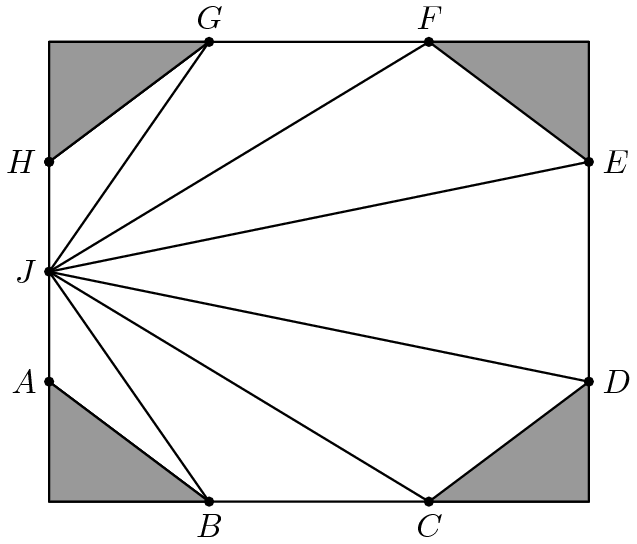
\includegraphics[width = 63.6mm]{img/fig0.png}
\end{center}